\begin{figure}[H]
    \centering
    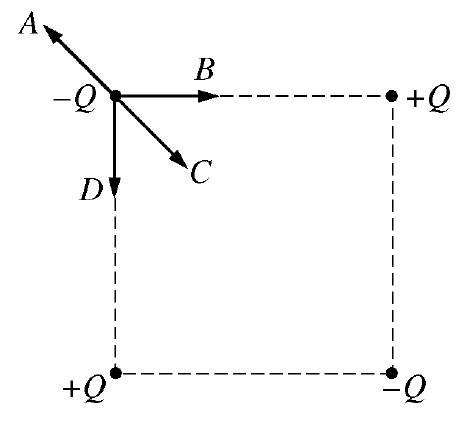
\includegraphics[scale=0.5]{images/35.png}
\end{figure}

% Multiple Choice Question 35
\begin{questions}\setcounter{question}{34}\question
Four point charges of equal magnitude but different signs are arranged on the corners of a square as shown above. Which of the vectors shown represents the direction of the net force acting on the charge at the upper left-hand corner of the square due to the other charges?

\begin{choices}
\choice $A$
\choice $B$
\choice $C$
\choice $D$
\choice It has no direction because the force is zero.
\end{choices}\end{questions}
